% This file was created with tikzplotlib v0.10.1.
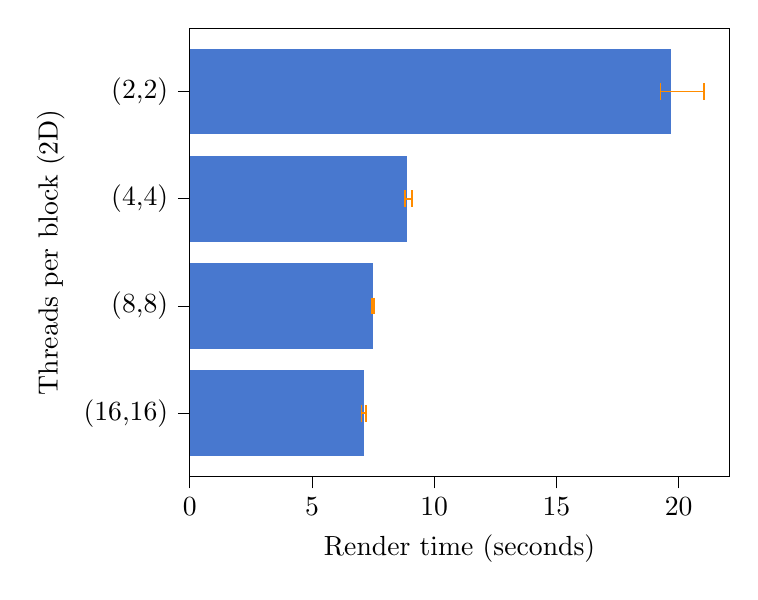
\begin{tikzpicture}

\definecolor{darkgray176}{RGB}{176,176,176}
\definecolor{darkorange}{RGB}{255,140,0}
\definecolor{royalblue72120207}{RGB}{72,120,207}

\begin{axis}[
tick align=outside,
tick pos=left,
x grid style={darkgray176},
xlabel={Render time (seconds)},
xmin=0, xmax=22.07415,
xtick style={color=black},
y dir=reverse,
y grid style={darkgray176},
ylabel={Threads per block (2D)},
ymin=-0.59, ymax=3.59,
ytick style={color=black},
ytick={0,1,2,3},
yticklabels={{(2,2)},{(4,4)},{(8,8)},{(16,16)}}
]
\draw[draw=none,fill=royalblue72120207] (axis cs:0,-0.4) rectangle (axis cs:19.675,0.4);
\draw[draw=none,fill=royalblue72120207] (axis cs:0,0.6) rectangle (axis cs:8.892,1.4);
\draw[draw=none,fill=royalblue72120207] (axis cs:0,1.6) rectangle (axis cs:7.504,2.4);
\draw[draw=none,fill=royalblue72120207] (axis cs:0,2.6) rectangle (axis cs:7.136,3.4);
\path [draw=darkorange, semithick]
(axis cs:19.255,0)
--(axis cs:21.023,0);

\path [draw=darkorange, semithick]
(axis cs:8.795,1)
--(axis cs:9.097,1);

\path [draw=darkorange, semithick]
(axis cs:7.454,2)
--(axis cs:7.529,2);

\path [draw=darkorange, semithick]
(axis cs:7.03,3)
--(axis cs:7.206,3);

\addplot [semithick, darkorange, mark=|, mark size=3, mark options={solid}, only marks]
table {%
19.255 0
8.795 1
7.454 2
7.03 3
};
\addplot [semithick, darkorange, mark=|, mark size=3, mark options={solid}, only marks]
table {%
21.023 0
9.097 1
7.529 2
7.206 3
};
\end{axis}

\end{tikzpicture}
